In this section project outcomes are described.
Outcomes description includes the specifications of concrete functional requirements implemented along with the
graphic user interface screenshots.
Function requirements could be found at annex~\ref{ch:list-of-functional-requirements}.
We begin from the messenger's start page and continue further with user contacts component and user settings component.
\begin{figure}[H]
    \centering
    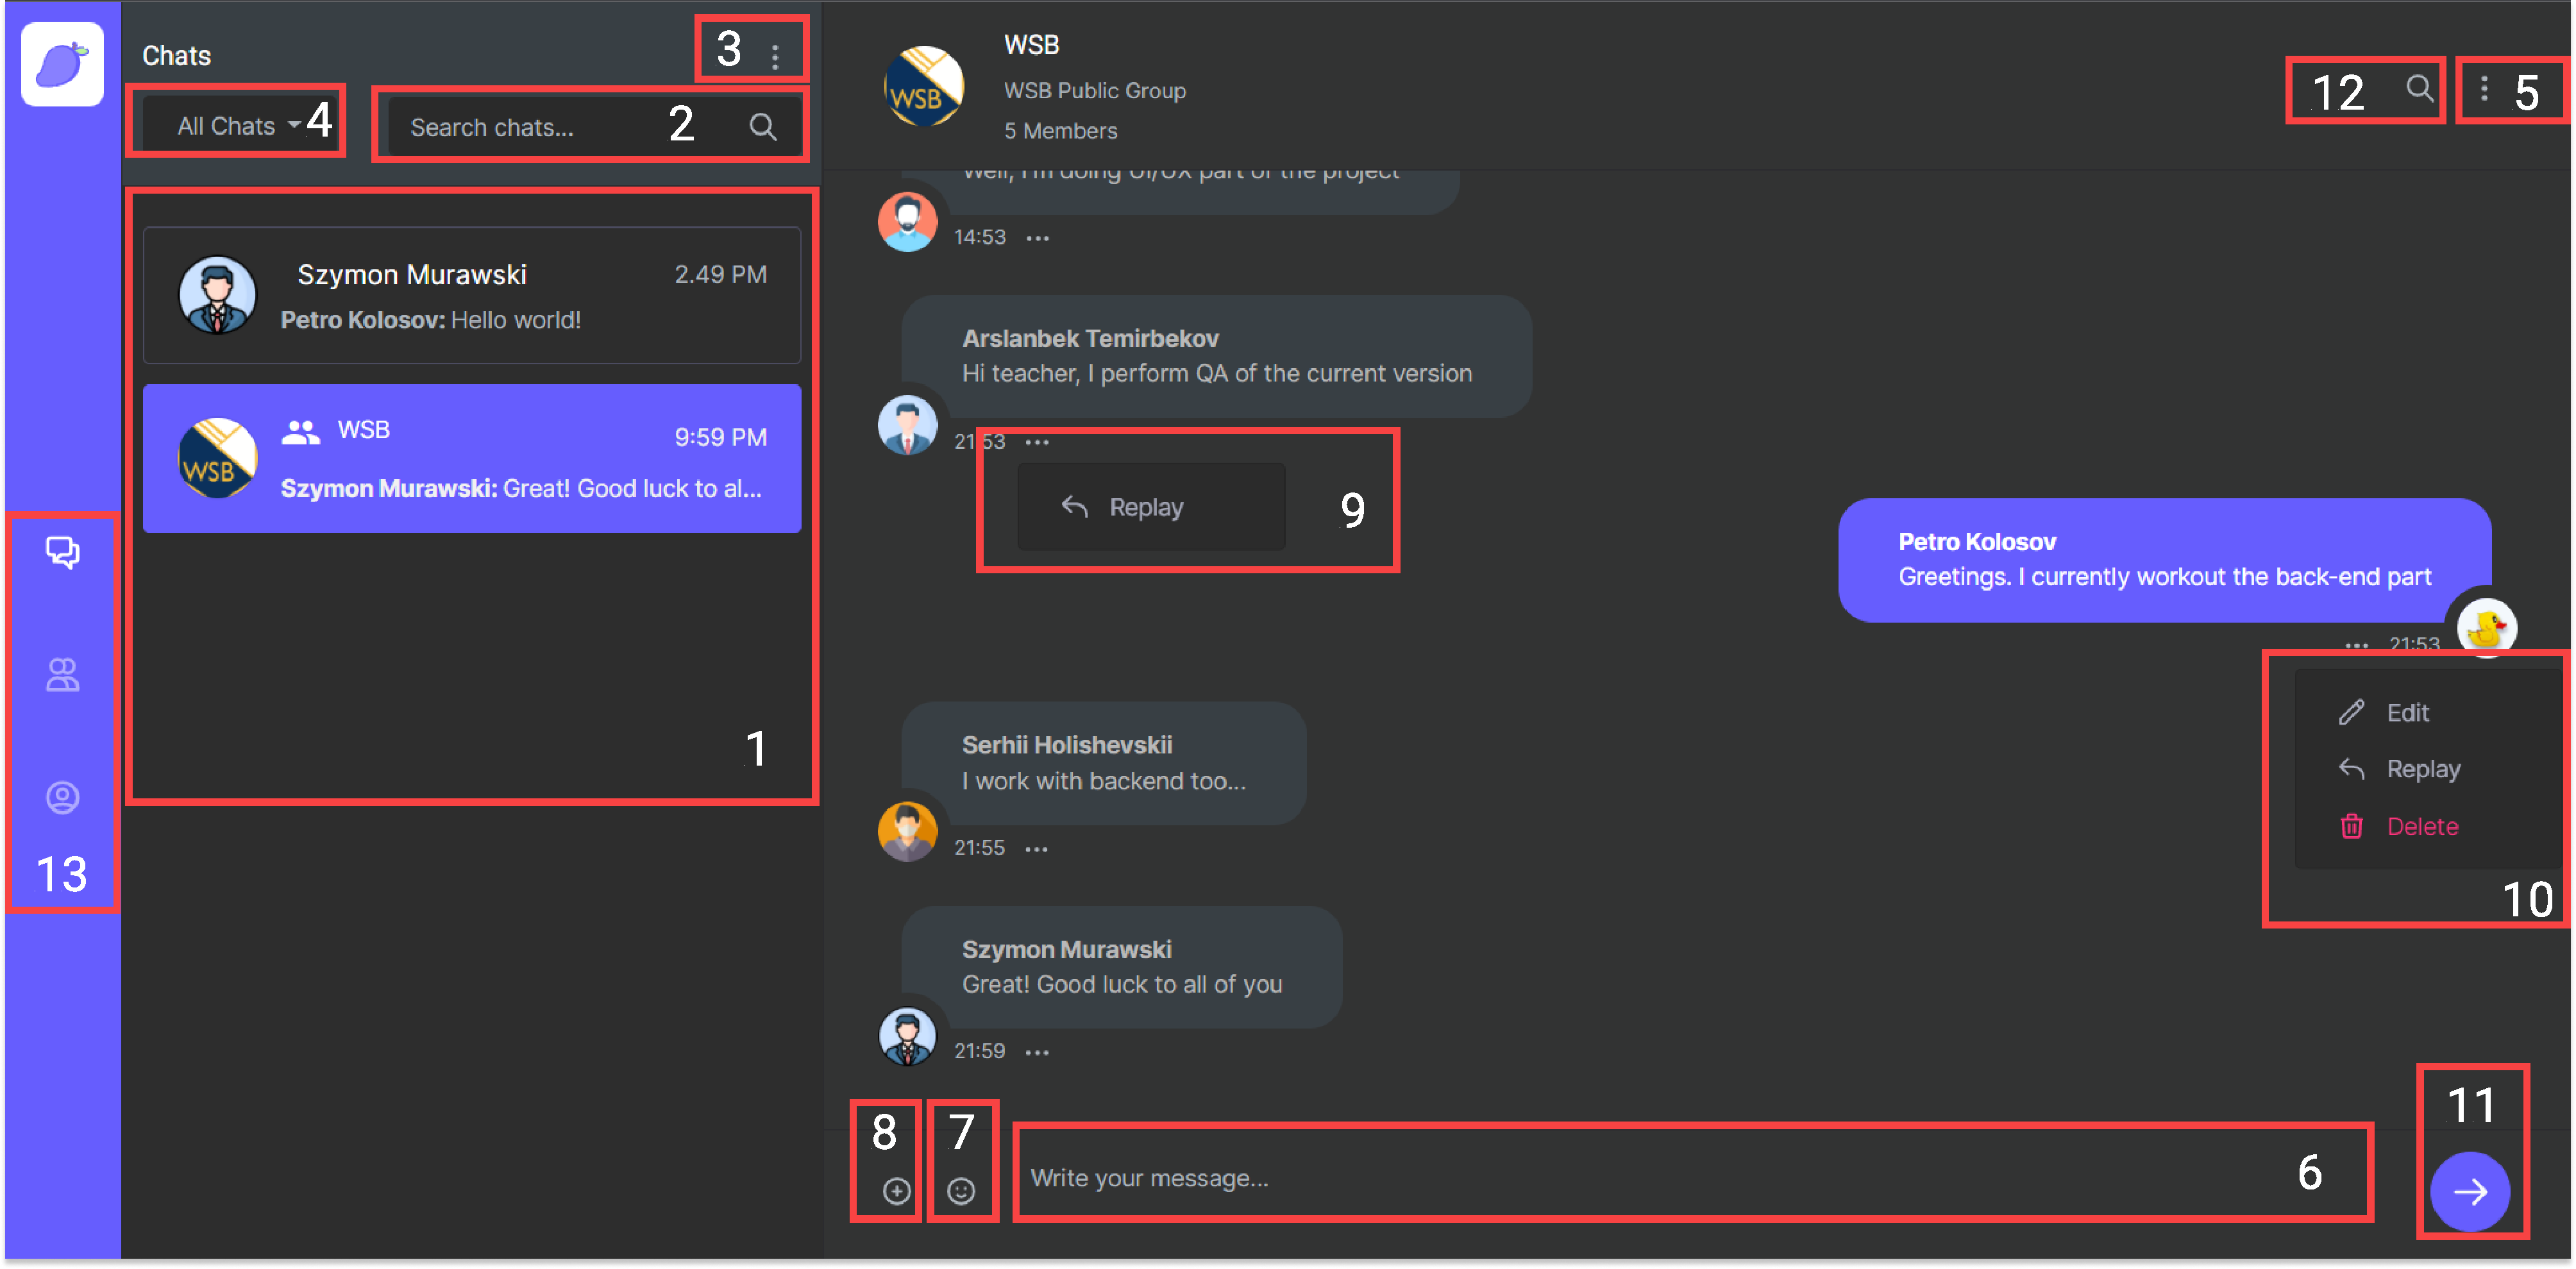
\includegraphics[width=1\textwidth]{Pictures/09_Messenger_startpage}
    \caption{Start page component screenshot.}\label{fig:figure5}
\end{figure}

\begin{enumerate}
    \item Element responsible for getting user's chats list so that functional requirement \textit{"As an authorized user,
        I want to view a message history of particular chat or group so that I see a list of my active chats on the UI"}
    is satisfied.
    \item Element responsible for searching chats by display name and displaying it so that functional requirements
    \begin{itemize}
        \item \textit{"As an authorized user, I want to search public groups by title so that I enter display name to specified field,
            click button "Search chats" and see results"}
        \item \textit{"As a registered user, I want to join public groups so that I click button "Join group"to join the group"}
    \end{itemize}
    are satisfied.
    \item Element responsible for creating groups so that functional requirement
    \textit{"As a registered user, I want to tap "Create channel" so that I create a new channel of the one of the types:
    Private channel, Public channel, Readonly channel"} is satisfied.
    \item Element responsible for filtering chats so that functional requirement \textit{"As an authorized user,
        I want to filter a message history of particular chat or group so that I see a filtered list of my active
        chats on the UI"} is satisfied.
    \item Element responsible for archiving and leaving from the particular chat, so that functional requirements
    \begin{itemize}
        \item \textit{"As registered user, I want to tap "Leave" so that I leave from specified chat or channel"}
        \item \textit{"As a registered user, I want to tap "Archive" so that I archive the specified chat or channel"}
        \item \textit{"As a registered user, I want to tap "Un-archive" so that I un-archive the specified archived chat or channel"}
    \end{itemize}
    are satisfied.
    \item Element responsible for entering the text and sending a message by enter, so that functional requirement
    \textit{"As an authorized user, I want to send a text message so that other members of the group see the message I sent"}
    is satisfied.
    \item Element responsible for adding emoji to message, so that functional requirement
    \textit{"As an authorized user, I want to add an emoji to the message so that other members of the group
    see the message with emoji I sent"} is satisfied.
    \item Element responsible for adding attachments to the message, so that functional requirement
    \textit{"As an authorized user, I want to add an attachment to the message so that other members of the group see the
    message with attachment I sent"} is satisfied.
    \item Element responsible for replying to message, so that functional requirement
    \textit{"As registered user, I want tap "Reply" so that I want reply to the particular message"} is satisfied.
    \item Element responsible for editing and deleting a message so that functional requirements
    \begin{itemize}
        \item \textit{"As an authorized user, I want to tap "Edit" on my message so that other members of the group
        see the message I edited"}
        \item \textit{"As an authorized user, I want to tap "Delete" on my message so that my message is deleted for
        all members of the group"}
    \end{itemize}
    are satisfied.
    \item Element responsible for sending message if message text field is not empty so that functional requirement
    \textit{"As an authorized user, I want to send a text message so that another user sees my message"}
    is satisfied.
    \item Element responsible for searching messages in the particular chat so that functional requirement
    \textit{"As an authorized user, I want to search messages in particular chat so that I see the results in
    messages window of the chat"} is satisfied.
    \item Element responsible for navigation about main page, contacts page and personal information page so that
    functional requirement
    \textit{"As an authorized user, I want to navigate between the pages so that there is a menu on the UI"} is satisfied.
\end{enumerate}

\begin{figure}[H]
    \centering
    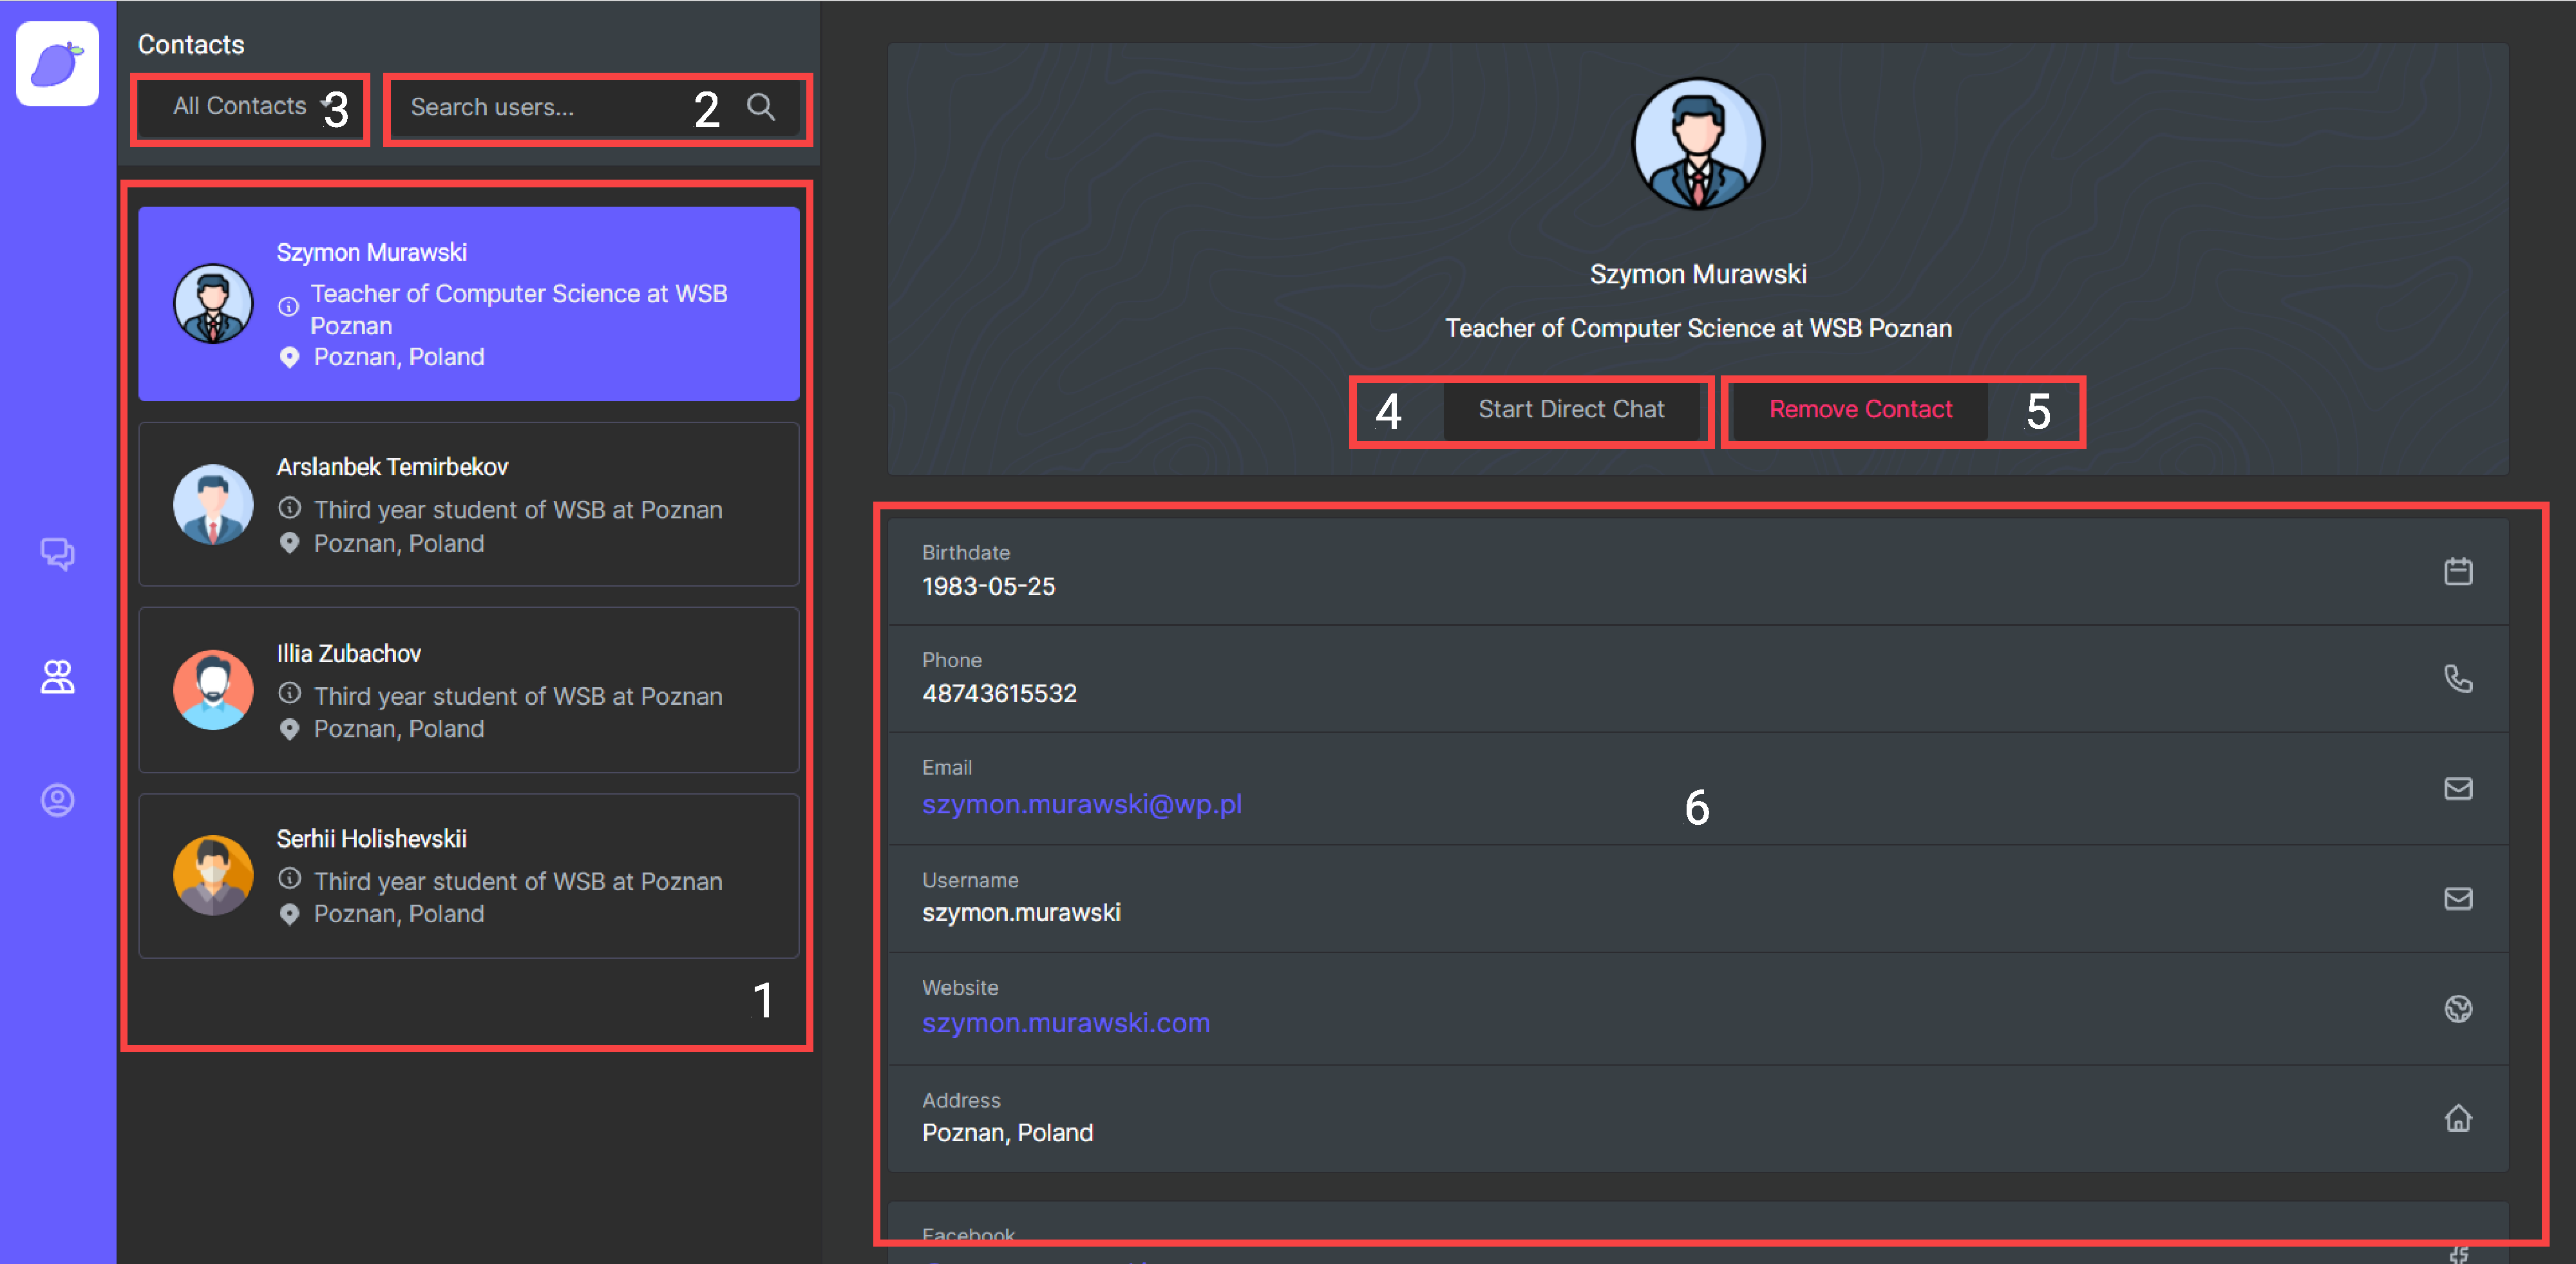
\includegraphics[width=1\textwidth]{Pictures/10_Messenger_manage_contacts}
    \caption{Manage contacts component screenshot.}\label{fig:figure10}
\end{figure}
\begin{enumerate}
    \item Element responsible for output user's contacts so that functional requirement
    \textit{"As an authorized user, I want to see my contact list so that there is a list of users
    who are my contacts"} is satisfied.
    \item Element responsible for searching users so that functional requirement
    \textit{"As an authorized user, I want to search users so that I write user display name or phone number
    of e-mail address to specified input, click "Search user" button and see
    results"} is satisfied.
    \item Element responsible for filtering contacts so that functional requirement
    \textit{"As an authorized user, I want to search users so that I write user display name or phone number of e-mail
    address to specified input, click "Search user" button and see results"} is satisfied.
    \item There is a button, clicking on which you can start chat with a specific user, so that functional requirement
    \textit{"As a registered user, I want to tap "Start direct chat" so that I create a new direct
    chat with specified user"} is satisfied.
    \item Element responsible for deleting user form contacts so that functional requirement
    \textit{"As an authorized user, I want to remove the user from my contact list so that I click "Remove contact"
    button on user profile and remove him from my contact list"} is satisfied.
    \item Element responsible for the output specified user's info so that functional requirement
    \textit{"As an authorized user, I want to tap on specified contact so that I want see user's information"}
    is satisfied.
\end{enumerate}

\begin{figure}[H]
    \centering
    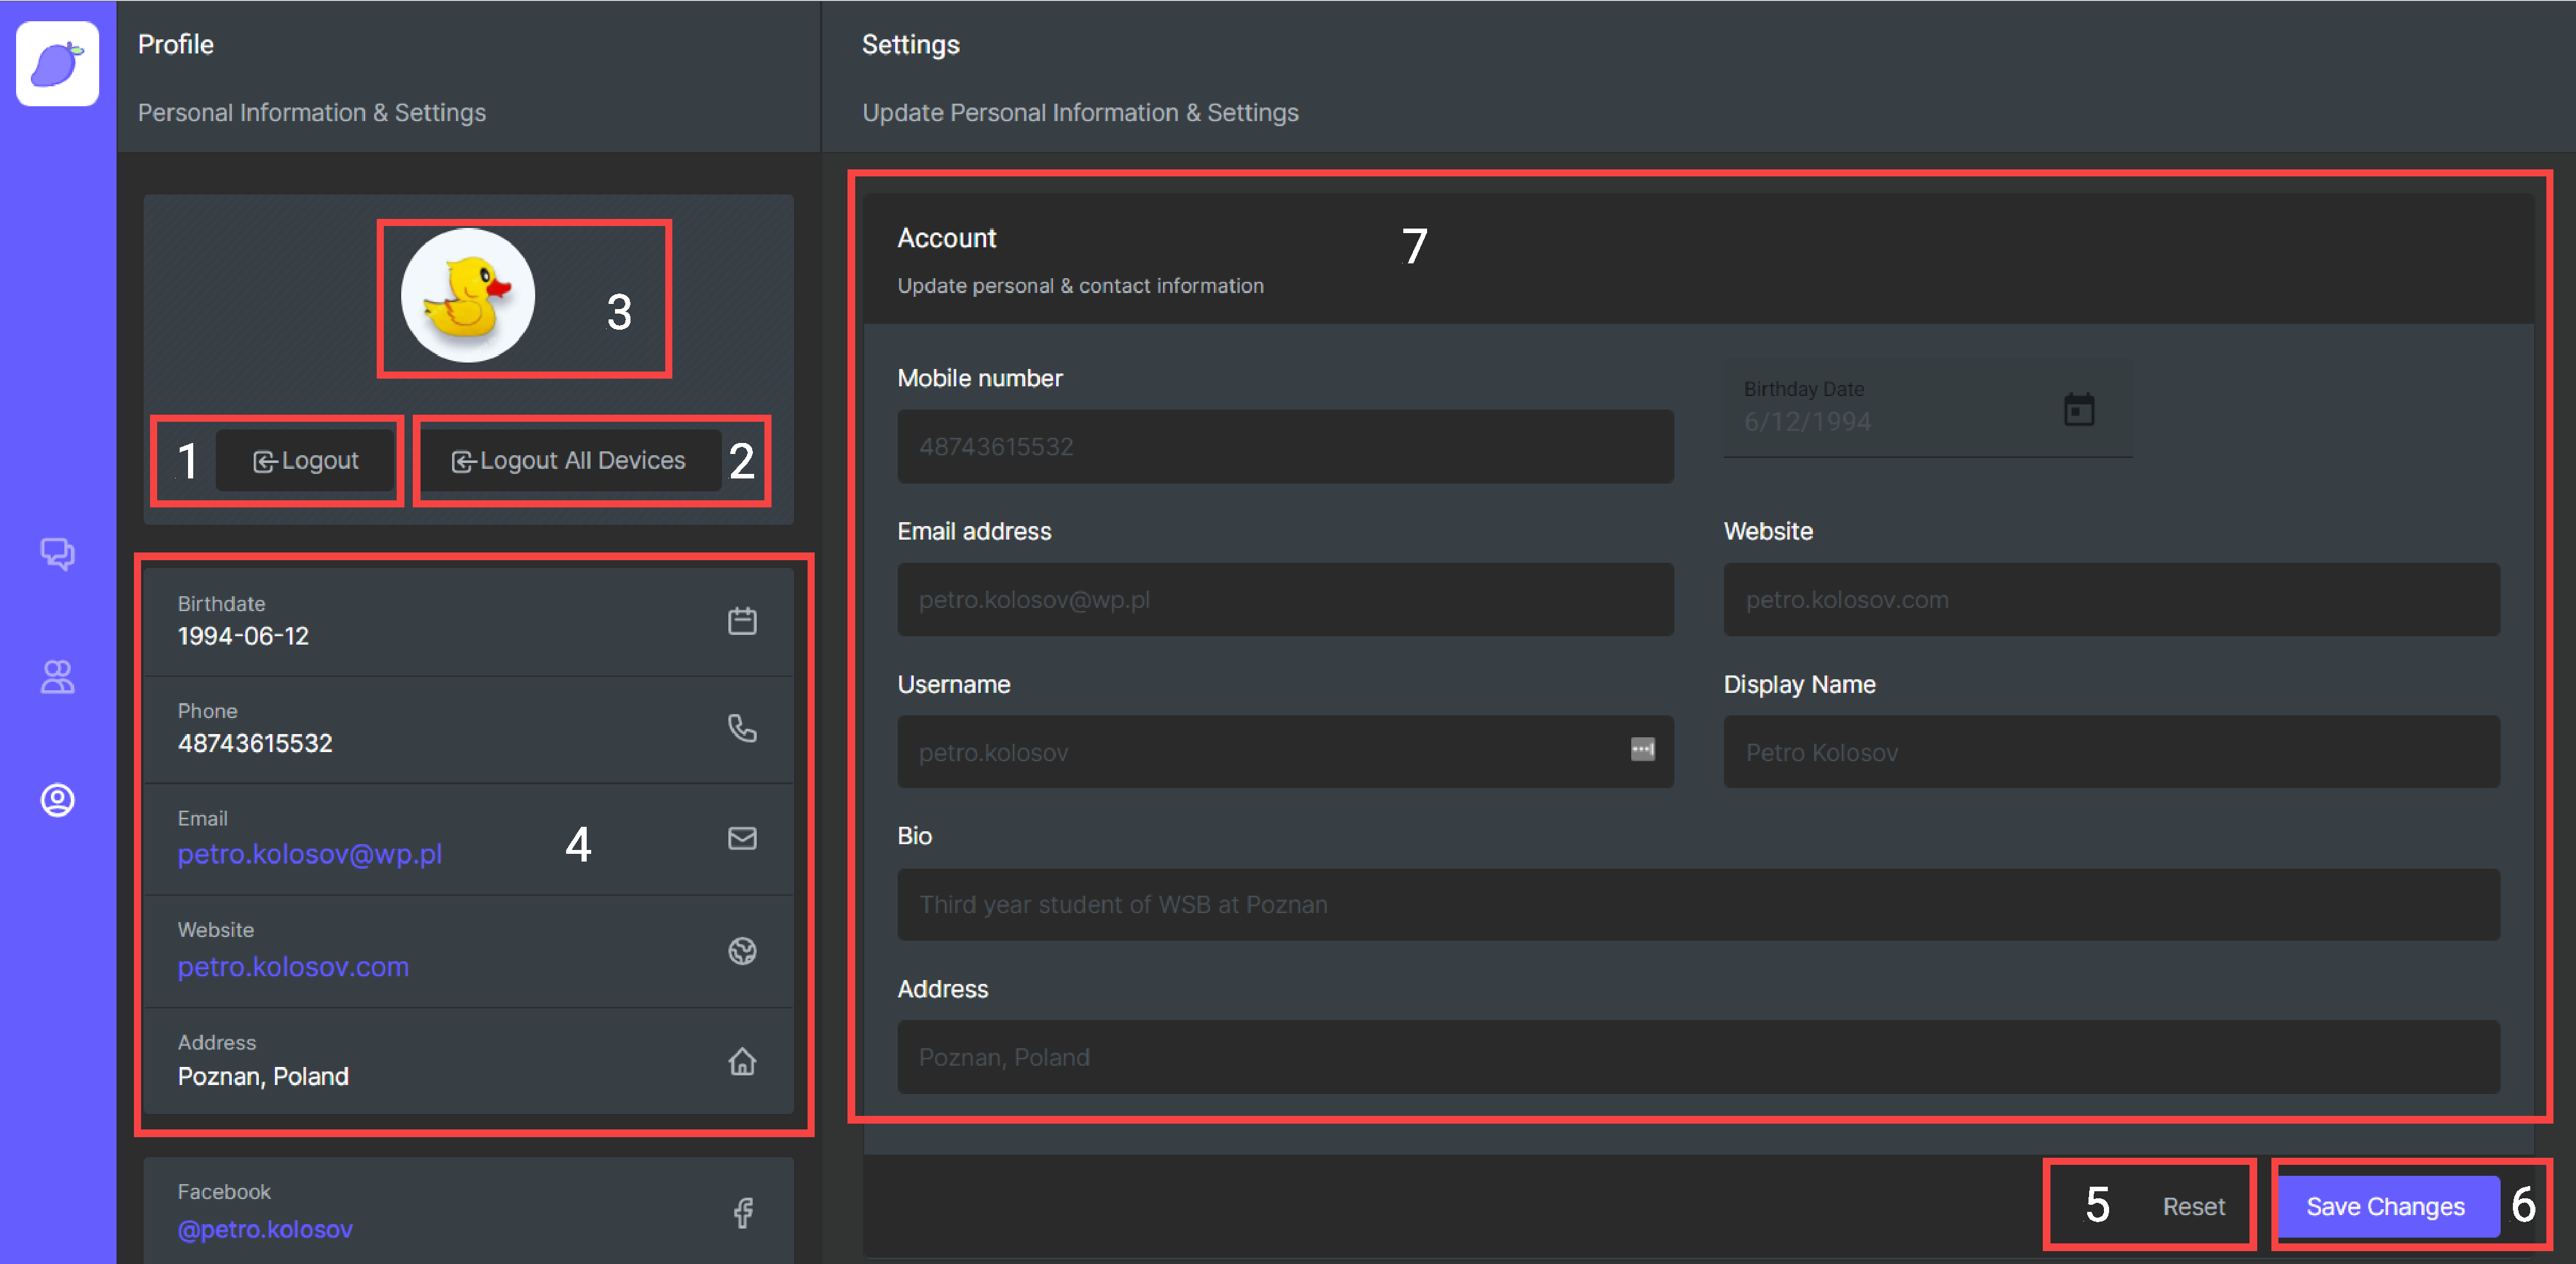
\includegraphics[width=1\textwidth]{Pictures/11_Messenger_account_settings}
    \caption{Account settings component screenshot.}\label{fig:figure11}
\end{figure}
\begin{enumerate}
    \item Element responsible for log out from specified device so that functional requirement
    \textit{"As an authorized user, I want to tap "Logout" button so that current device
    will be logged out from the system"} is satisfied.
    \item Element responsible for log out from all devices so that functional requirement
    \textit{"As an authorized user, I want to tap "Logout all" button so that all my authorized devices will be
    logged out from the system"} is satisfied.
    \item Element responsible for output user's avatar so that functional requirement
    \textit{"As an authorized user, I want to navigate to personal information page so that
    I want see my profile picture"} is satisfied.
    \item Element responsible for output user's information so that functional requirement
    \textit{"As an authorized user, I want to navigate to personal information page so that I want see my
    personal information"} is satisfied.
    \item Element responsible for reset updated personal information so that functional requirement
    \textit{"As an authorized user, I want to tap "Reset" so that I want reset my updated (not saved)
        personal information"} is satisfied.
    \item Element responsible for saving personal information so that functional requirement
    \textit{"As an authorized user, I want save my updated personal information so that users see it"}
    is satisfied.
    \item Element responsible for changing personal information so that functional requirement
    \textit{"As an authorized user, I want to update my personal information in profile settings so that other users
    my updated personal information"} is satisfied.
\end{enumerate}
Finally, we attach the list of technologies was used during an implementation of the project.
List of technologies are separated by categories is as follows
\begin{itemize}
    \item \textbf{SDK}: \href{https://dotnet.microsoft.com/download/dotnet/5.0}{.NET Core 5.0}
    \item \textbf{Backend:} \href{https://dotnet.microsoft.com/apps/aspnet}{ASP.NET Web API}
    \item \textbf{Database}
    \begin{itemize}
        \item SQL Database: \href{https://www.postgresql.org/}{PostgreSQL 13}
        \item ORM: \href{https://www.nuget.org/packages/Microsoft.EntityFrameworkCore/5.0.7?_src=template}{Entity Framework Core 5.0.7}
        \item PostgreSQL Provider: \href{https://www.nuget.org/packages/Npgsql.EntityFrameworkCore.PostgreSQL/5.0.7?_src=template}{Npgsql.EntityFrameworkCore.PostgreSQL 5.0.7}
    \end{itemize}
    \item \textbf{Authorization}
    \begin{itemize}
        \item JWT Library: \href{https://www.nuget.org/packages/System.IdentityModel.Tokens.Jwt}{System JWT 6.8.0}
        \item JWT Library: \href{https://www.nuget.org/packages/System.IdentityModel.Tokens}{System Tokens 6.11.1}
        \item JWT Bearer: \href{https://www.nuget.org/packages/Microsoft.AspNetCore.Authentication.JwtBearer/5.0.7?_src=template}{Microsoft Jwt Bearer 5.0.7}
    \end{itemize}
    \item \textbf{Business Logic}
    \begin{itemize}
        \item \href{https://www.nuget.org/packages/MediatR/9.0.0?_src=template}{MediatR 9.0.0}
        \item \href{https://www.nuget.org/packages/FluentValidation/10.2.3?_src=template}{Fluent Validation 10.2.3}
        \item \href{https://www.nuget.org/packages/AutoMapper/}{AutoMapper 10.1.1}
    \end{itemize}
    \item \textbf{Presentation}
    \begin{itemize}
        \item Documentation: \href{https://www.nuget.org/packages/Swashbuckle.AspNetCore/5.6.3?_src=template}{Swashbuckle 6.1.4}
        \item Realtime Communication: \href{https://www.nuget.org/packages/Microsoft.AspNet.SignalR/}{SignalR 2.4.2}
        \item Frontend Development: \href{https://angular.io/guide/setup-local}{Angular 11.2.7}
        \item Desktop Development: ElectronJS framework.
        \item Mobile Development:
    \end{itemize}
    \item \textbf{Unit and Integration Testing}
    \begin{itemize}
        \item Testing Framework: \href{https://www.nuget.org/packages/NUnit/}{NUnit 3.13.1}
        \item Testing Auxiliary: \href{https://www.nuget.org/packages/Moq/}{Moq 4.16.1}
        \item Testing Auxiliary: \href{https://www.nuget.org/packages/FluentAssertions}{FluentAssertions 6.0.0}
    \end{itemize}
    \item \textbf{Static Code Analysis}: \href{https://www.sonarqube.org/downloads/}{SonarQube 8.9.2 LTS Community Edition}
    \item \textbf{Containerization}: \href{https://docs.docker.com/desktop/windows/install/}{Docker 3.6.0}
    \item \textbf{Continuous Integration}: \href{https://docs.github.com/en/actions}{GitHub Actions}, Heroku, Azure
    \item \textbf{Programming languages}: C\#, SQL, TypeScript
    \item \textbf{Tools}: Microsoft Visual Studio, JetBrains Rider, Visual Studio Code, WebStorm.
\end{itemize}